\subsection{Session 4, Exercise 2}

\lineparagraph{Exercise}

Consider

\begin{align*}
S \rightarrow& AS|A\\
A \rightarrow& 0A1|01
\end{align*}

\begin{enumerate}[(a)]
\item Give a parse tree and a leftmost derivation for word 01010011.
\item Determine the language generated by this grammar.
\end{enumerate}

\lineparagraph{Solution}

a)

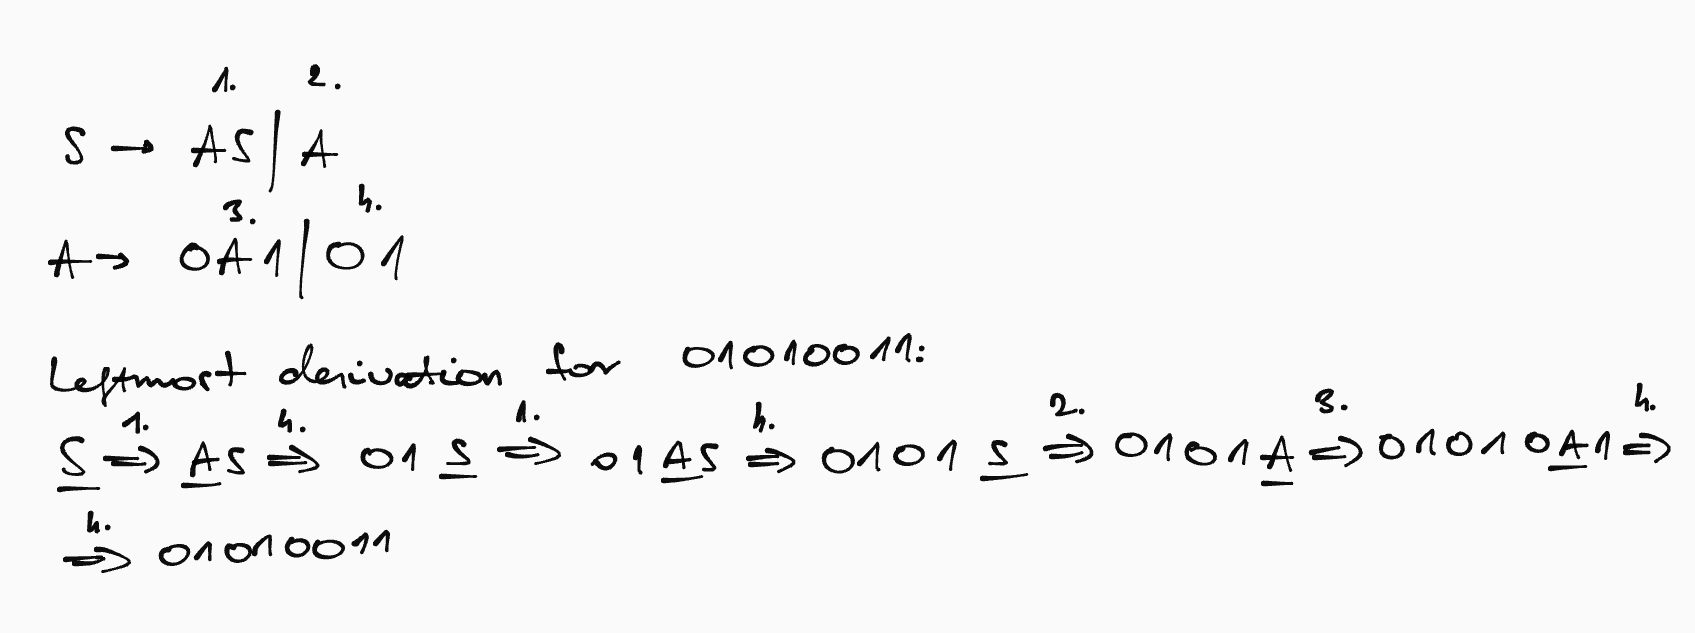
\includegraphics[width=\linewidth]{04/4_2_a_1.png}
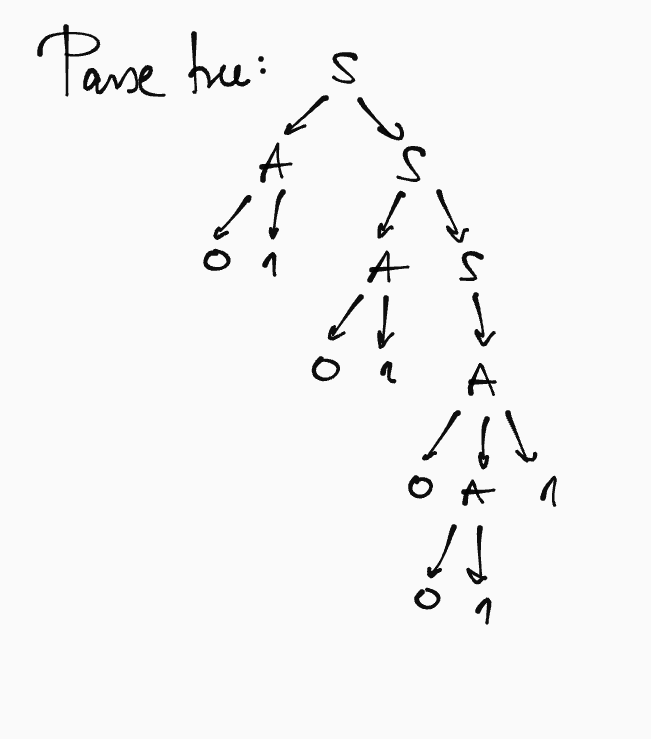
\includegraphics[width=\linewidth]{04/4_2_a_2.png}

b)

From $A$ we can derive the following set of words: $L_A = \{0^n1^n | n\geq{}1\}$, and $S$ allows for conatenating $A$'s, so $L_S=\{0^{n_1}1^{n_1}0^{n_2}1^{n_2}\dots0^{n_k}1^{n_k} | k\geq{}1, n_1,n_2\dots,n_k\geq{}1\}$.